Il presente lavoro di tesi ha l'obiettivo di migliorare il sistema di monitoraggio delle presenze dell'applicazione ZConnect di Zucchetti S.P.A.. Inizialmente è stata affrontata una fase di analisi per poter comprendere chi avrebbe utilizzato il sistema di monitoraggio delle presenze, qual'era lo stato attuale del sistema, nella versione Android e iOS, e per capire quali requisiti doveva soddisfare l'implementazione, come descritto nelle Sezioni 2.1, 2.2 e 2.3 di questo capitolo.

Durante l'analisi, è stata posta particolare attenzione a garantire un supporto di facile e immediata consultazione per gli utenti, soprattutto per agevolare la registrazione della presenza nel luogo designato. L'analisi ha contribuito a identificare gli obiettivi principali del nuovo sistema, nonché i requisiti funzionali e non funzionali che dovevano essere soddisfatti.

L'obiettivo di questo capitolo è presentare in dettaglio i risultati dell'analisi condotta, evidenziando le sfide affrontate, le conclusioni tratte e come tali risultati hanno orientato l'implementazione del sistema di monitoraggio delle presenze in azienda basato sulla geolocalizzazione.

\section{Analisi degli attori}

Gli utenti che utilizzeranno la funzionalità per registrare le proprie presenze in azienda sono i dipendenti dell'azienda a cui è venduta l'applicazione ZConnect, in particolar modo i dipendenti dell'Azienda X. I dipendenti dell'azienda X che utilizzeranno questa funzionalità sono in maggior parte degli operai edili che operano in aree di lavoro molto estese sul territorio. Ogni dipendente avrà accesso all'applicazione tramite un account personale, che gli consentirà di effettuare le operazioni di timbratura, utilizzando una mappa come supporto nel raggiungimento dell'area di lavoro, sarà inoltre possibile per gli utenti consultare il proprio storico delle presenze.

Gli utenti, quindi, hanno la necessità di utilizzare questa funzionalità in modo immediato, per poter registrare la propria presenza in azienda ed iniziare il loro lavoro. Hanno, inoltre, la necessità di poter consultare una mappa dinamica in cui siano facilmente identificabili la propria posizione e l'area in cui poter registrare la propria presenza più vicina a loro.

\section{Analisi del sistema esistente}\label{Analisi_sistema}

Come già menzionato nell'Introduzione l'applicazione ZConnect è sviluppata sia per Android \cite{Android}, utilizzando Java \cite{Java} e Kotlin \cite{Kotlin}, che per iOS \cite{iOS}, utilizzando Swift \cite{Swift}. Questo duplice sviluppo comporta delle differenze di implementazione, in quanto la stessa applicazione viene sviluppata per due sistemi operativi differenti utilizzando linguaggi differenti.

In entrambe le versioni di ZConnect per realizzare il servizio di monitoraggio delle presenze, a ciascun utente viene associata una lista di luoghi geografici all'interno dei quali è abilitato a registrare la propria presenza. Questi luoghi sono modellati come geofence, che rappresentano un perimetro virtuale attorno a un luogo specifico \cite{GeoFence}. L'associazione tra utente e luoghi geografici è effettuata dal server, all'applicazione viene inviata la lista dei luoghi associata all'utente.

All'interno dell'applicazione, un geofence è modellato attraverso un'interfaccia chiamata IGeoFence. L'interfaccia IGeoFence è identica sia nell'ambito di Android che di iOS. Questa interfaccia specifica il tipo di geofence, che può essere poligonale, circolare, quadrato, o anche di tipo nullo. Quest'ultima opzione è stata introdotta per modellare i tag NFC utilizzati in altre sezioni dell'applicazione, assimilandoli a geofence. L'interfaccia IGeoFence include anche una serie di metodi ``get" per recuperare informazioni come il tipo di geofence, il centro del geofence e le coordinate geografiche. In particolare, risultano fondamentali la latitudine e la longitudine massima e minima, poiché, nei casi d'uso attuali, tutti i geofence sono di tipo quadrato. Avendo a disposizione le latitudini e le longitudini minime e massime, è possibile delineare il perimetro dello spazio geografico modellato tramite il geofence con quattro punti.

Tramite un algoritmo, ZConnect verifica che la posizione dell'utente sia all'interno del perimetro di uno dei geofence associati all'utente. ZConnect esegue questo algoritmo quando l'utente è sulla schermata in cui può effettuare una timbratura ogni volta che rileva un cambio di posizione del device.
Gli utenti si possono trovare in due situazioni, all'esterno di un'area geografica preposta per la registrazione della presenza ed all'interno di un'area geografica preposta per la registrazione della presenza. Se si trovano all'interno di un'area geografica proposta per la registrazione della presenza, potranno effettuare la timbratura. Se invece si trovano all'esterno non potranno effettuare la registrazione della presenza.
In entrambi i casi, per gli utenti è possibile aprire una mappa. Nel caso in cui l'utente si trovi all'interno di un area in cui effettuare la timbratura, l'applicazione mostra il geofence indicato come valido per la timbratura centrando la mappa sul centro del geofence, con un marker, rosso per entrambe le versioni dell'applicazione, al centro dello stesso per indicare la posizione. Invece, nel caso in cui l'utente si trovi fuori da un'area in cui può effettuare la timbratura, l'applicazione mostra la mappa centrata sulla posizione dell'utente con un marker, rosso per la versione Android e blu per la versione iOS, che indicava la posizione dell'utente.

\begin{figure}[ht!]
    \begin{subfigure}{0.4\textwidth}
        \centering
        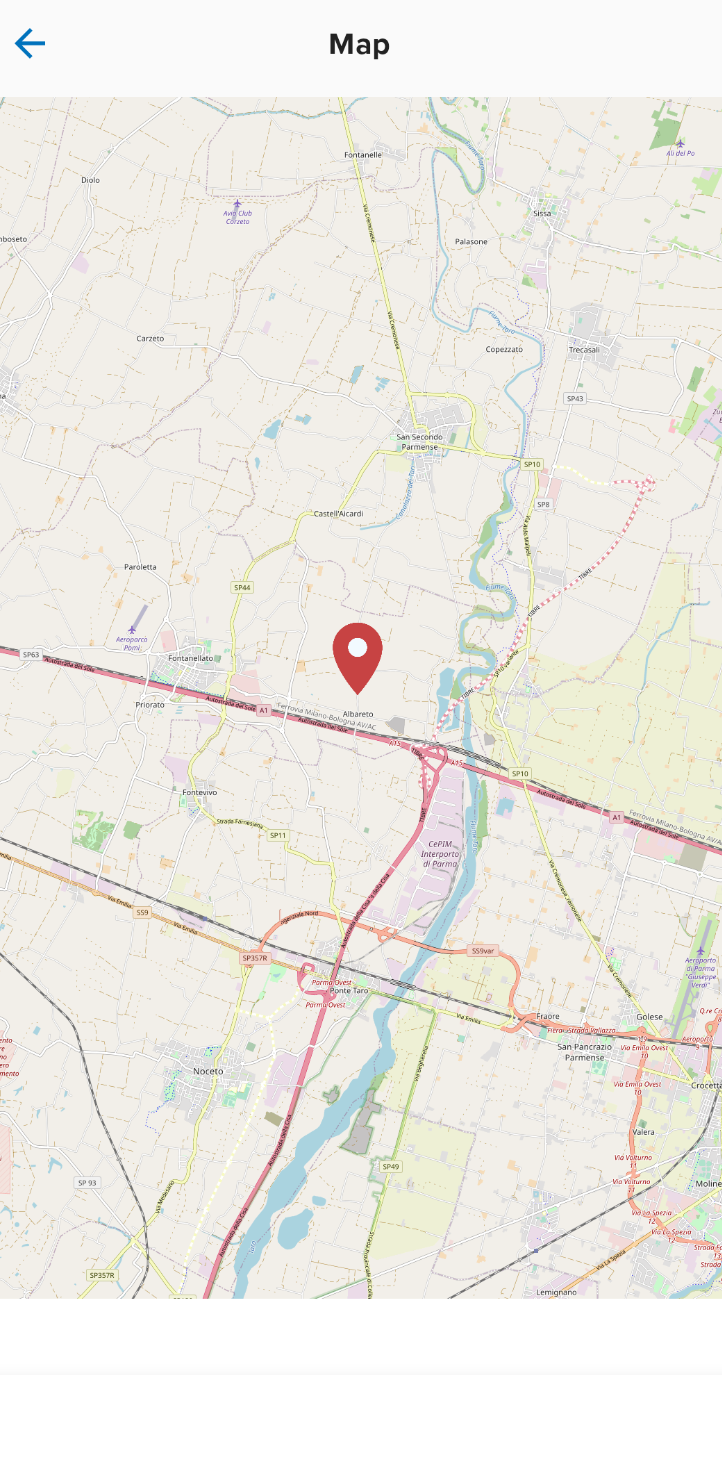
\includegraphics[width=\linewidth]{Immagini/vecchia_posizione_esterna.png}
        \caption{Mappa visualizzata quando l'utente è all'esterno di un geofence}
        \label{fig:vecchia_posizione_esterna_Android}
    \end{subfigure}
    \hspace{1cm} % Spazio orizzontale tra le immagini
    \begin{subfigure}{0.4\textwidth}
        \centering
        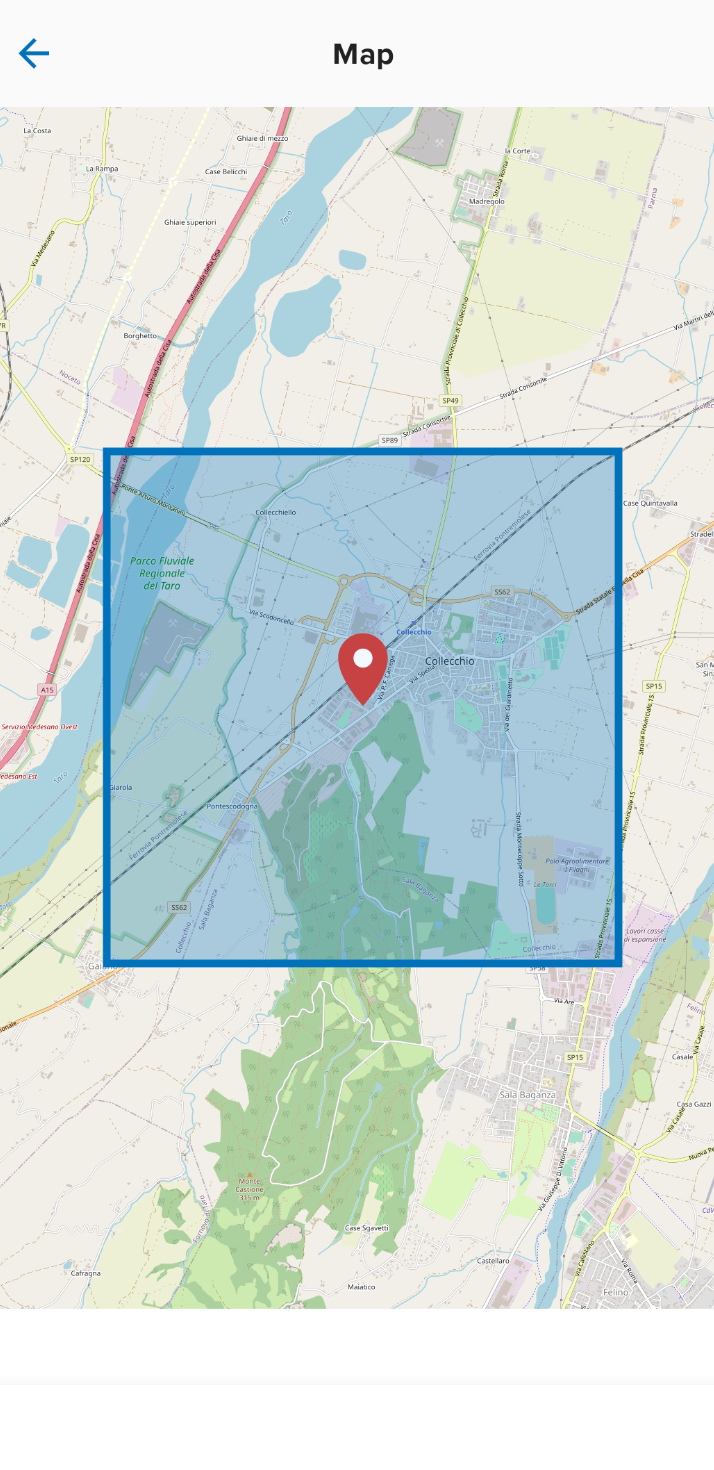
\includegraphics[width=\linewidth]{Immagini/vecchia_posizione_interna.png}
        \caption{Mappa visualizzata quando l'utente è all'interno di un geofence}
        \label{fig:vecchia_posizione_interna_Android}
    \end{subfigure}
    \caption{Mappa di ZConnect per Android}
    \label{fig:vecchia_mappa_android}
\end{figure}

\begin{figure}[ht!]
    \begin{subfigure}{0.4\textwidth}
        \centering
        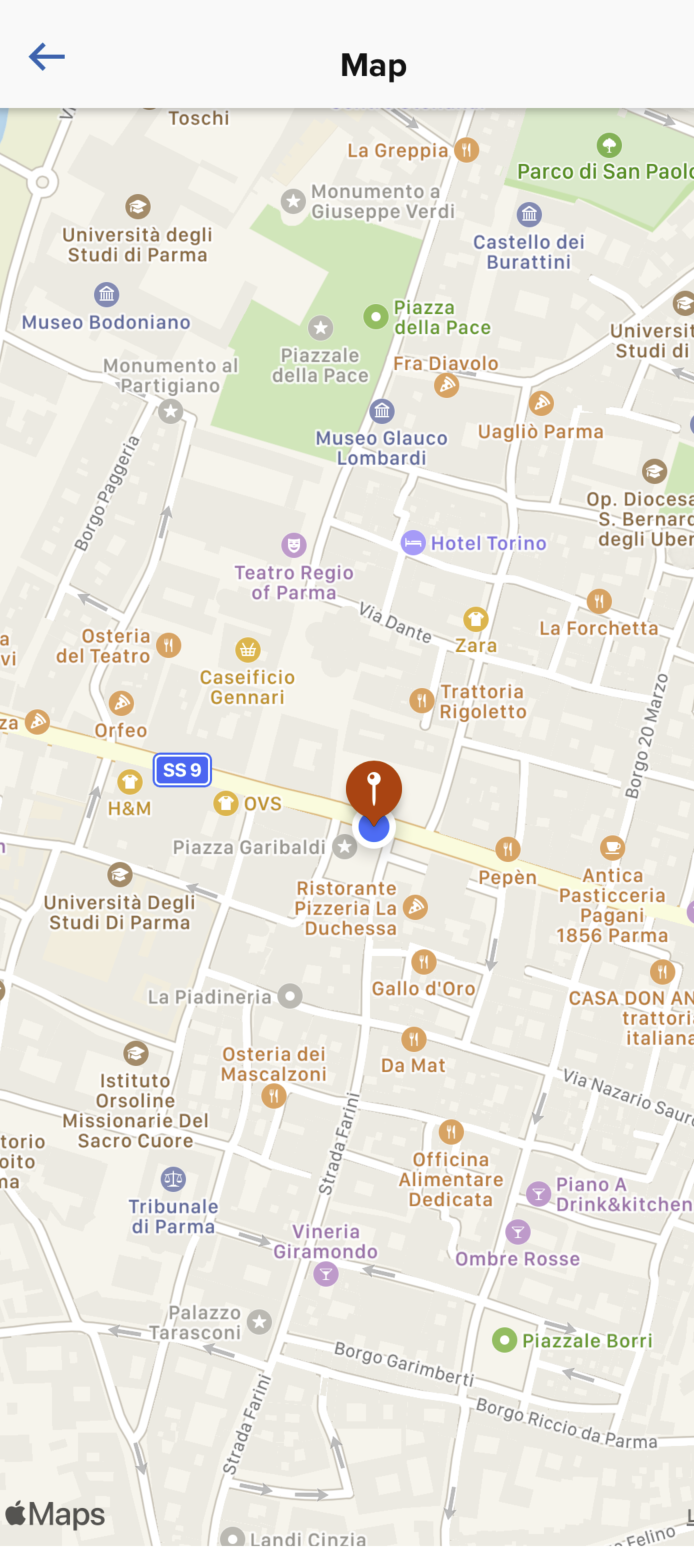
\includegraphics[width=\linewidth]{Immagini/vecchia_posizione_esterna_ios.png}
        \caption{Mappa visualizzata quando l'utente è all'esterno di un geofence}
        \label{fig:vecchia_posizione_esterna_iOS}
    \end{subfigure}
    \hspace{1cm} % Spazio orizzontale tra le immagini
    \begin{subfigure}{0.4\textwidth}
        \centering
        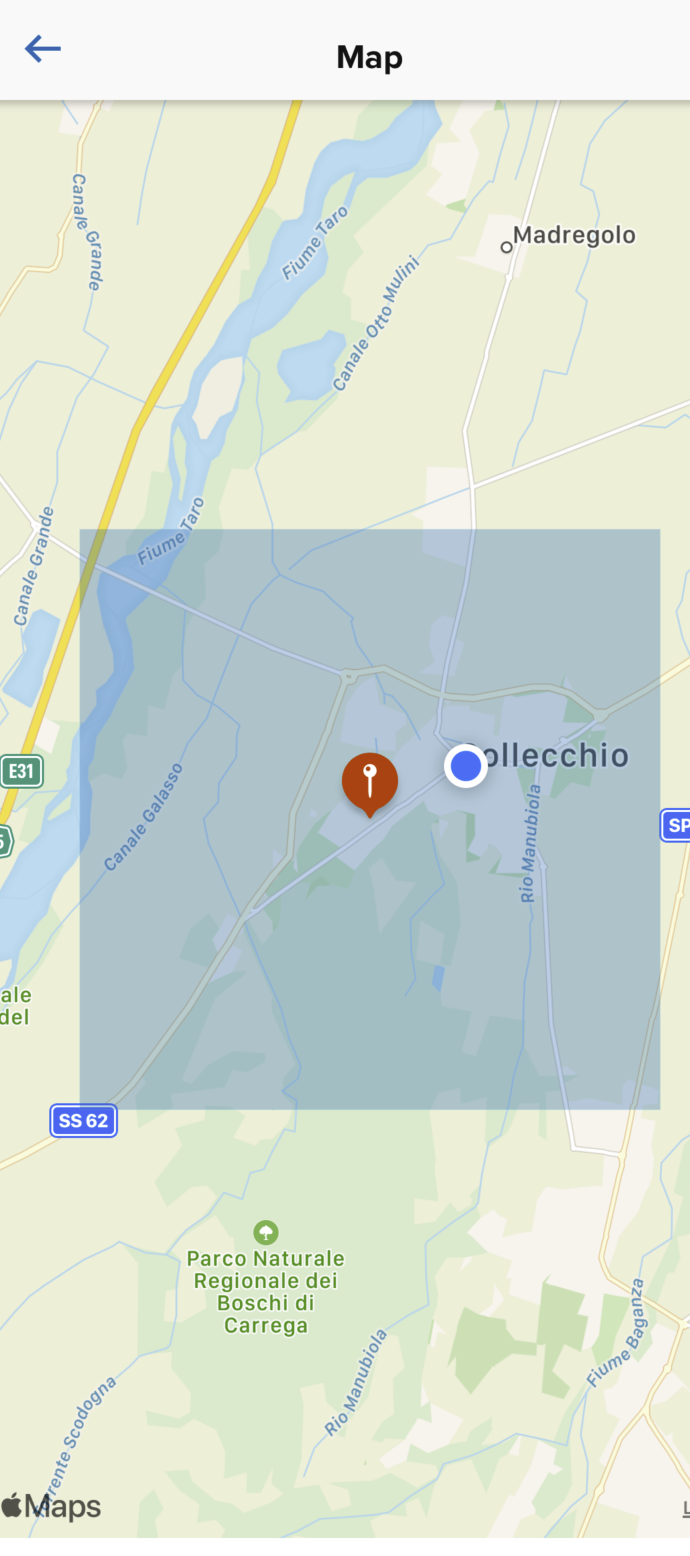
\includegraphics[width=\linewidth]{Immagini/vecchia_posizione_interna_ios.png}
        \caption{Mappa visualizzata quando l'utente è all'interno di un geofence}
        \label{fig:vecchia_posizione_interna_iOS}
    \end{subfigure}
    \caption{Mappa di ZConnect per iOS}
    \label{fig:vecchia_mappa_android_2}
\end{figure}

A causa del duplice sviluppo di ZConnect, l'implementazione delle mappe varia tra le due versioni.
Nella versione Android di ZConnect, viene utilizzata la libreria Osmdroid. Osmdroid è una libreria specifica per Android che offre strumenti per interagire con OpenStreetMap (OSM). OpenStreetMap (OSM) è un progetto collaborativo finalizzato a creare mappe del mondo a contenuto libero. Il progetto punta ad una raccolta mondiale di dati geografici, con scopo principale la creazione di mappe e cartografie \cite{OpenStreetMapWiki}.
Nel codice Android di ZConnect il fragment \cite{Fragment} che si occupa di mostrare la mappa è HRMapsOsmFragment. La mappa però nel fragment non viene gestita direttamente utilizzando i metodi forniti della libreria Osmdroid, ma viene utilizzata un'interfaccia IMapBinder, e la sua implementazione concreta OSMapBinder, che hanno lo scopo di esporre metodi per la gestione della mappa. L'interfaccia IMapBinder è stata progettata per poter garantire flessibilità per il futuro, in quanto è solamente l'implementazione concreta di IMapBinder ad utilizzare i metodi forniti dalla libreria delle mappe, rendendo così possibile cambiare la libreria in futuro senza dover modificare il codice dei fragment che mostrano la mappa.

Nella versione iOS di ZConnect, la visualizzazione della mappa è gestita utilizzando la libreria MapKit \cite{MapKitDoc}. La libreria MapKit è fornita direttamente da Apple e offre diverse funzionalità per l'integrazione delle mappe nelle applicazioni iOS.
A differenza di quanto fatto in Android, i metodi forniti dalla libreria MapKit vengono utilizzati direttamente nel ViewController \cite{ViewController} dedicato alla visualizzazione e all'interazione con la mappa, HRMapViewController. Alcuni dei metodi forniti dalla libreria MapKit permettono di impostare la regione di visualizzazione della mappa, aggiungere e personalizzare le annotazioni che rappresentano i luoghi di timbratura, e gestire le azioni dell'utente come lo zoom e lo spostamento sulla mappa.

\section{Problemi del sistema esistente}\label{Problemi_sistema}

Nell'implementazione precedente a questo lavoro di tesi del servizio di monitoraggio delle presenze di ZConnect, non veniva fornito un supporto adeguato agli utenti nel raggiungimento dell'area di lavoro, poiché, nel caso in cui l'utente si fosse trovato all'esterno di un'area di lavoro, la mappa non avrebbe mostrato con chiarezza la posizione dell'utente e la posizione dell'area di lavoro, fornendo un supporto inadeguato all'utente nel raggiungimento dell'area di lavoro, come è possibile vedere in Figura \ref{fig:vecchia_posizione_esterna_Android} e in Figura \ref{fig:vecchia_posizione_esterna_iOS}.

Questo limite creava una potenziale difficoltà per gli utenti nell'individuare con precisione l'area in cui dovevano registrare la propria presenza. L'assenza dei geofence sulla mappa impediva agli utenti di avere una visualizzazione diretta delle aree geografiche consentite per la timbratura, creando delle difficoltà nel raggiungimento del luogo di lavoro.

\section{Analisi dei requisiti}
La modifica del sistema di monitoraggio delle presenze, eseguita in questo lavoro di tesi, è stata guidata dalla necessità di soddisfare requisiti fondamentali. Il sistema rinnovato deve garantire all'utente la possibilità di registrare la propria presenza sul luogo di lavoro una volta raggiunto. Inoltre, l'utente deve avere la possibilità, sia che si trovi all'esterno di un luogo di lavoro, sia quando è all'interno, di visualizzare una mappa sulla quale sono rappresentati la propria posizione e tutti i luoghi di lavoro a lui associati, modellati come geofence. All'apertura della mappa, deve essere garantito un livello di zoom adeguato affinché l'utente possa visualizzare immediatamente la sua posizione e quella del luogo di lavoro più vicino.

Il marker che identifica la posizione dell'utente sulla mappa deve muoversi in tempo reale, seguendo gli spostamenti del dispositivo dell'utente, fornendo un feedback visivo immediato sulla direzione del movimento. Deve inoltre essere implementata una funzionalità "Follow-Me" che renda la mappa dinamica, garantendo che la posizione dell'utente sia sempre al centro della porzione di mappa visualizzata durante gli spostamenti.

\section{Analisi delle necessità}
La modifica del sistema di monitoraggio delle presenze deve essere progettata tenendo conto dell'utilizzo in movimento da parte degli utenti, pertanto richiede una connessione Internet per poter scaricare e visualizzare la mappa. Inoltre, è necessaria una connessione GPS per ricevere gli aggiornamenti di posizione e calcolare correttamente se il dispositivo si trova all'interno di un geofence abilitato per la timbratura o meno. È essenziale gestire accuratamente i casi in cui manca la connessione Internet o non è disponibile il segnale GPS.

Nel caso in cui il segnale GPS sia assente, il sistema deve essere in grado di gestire tale situazione. È importante fornire all'utente un feedback chiaro e tempestivo sullo stato della connessione GPS. Ad esempio, il sistema potrebbe visualizzare un messaggio di avviso o utilizzare indicazioni visive per comunicare che la posizione potrebbe non essere accuratamente rilevata.

Il sistema deve gestire in modo adeguato i casi in cui l'utente revoca o non concede i permessi per la localizzazione. In tali situazioni, è necessario fornire un'interfaccia chiara che guidi l'utente a concedere i permessi richiesti e spieghi l'importanza di tali autorizzazioni per il corretto funzionamento del sistema di monitoraggio delle presenze.

La corretta gestione delle connessioni Internet, del segnale GPS e dei permessi per la localizzazione è essenziale per garantire un'esperienza utente senza problemi e per consentire al sistema di funzionare in modo affidabile e preciso in diverse condizioni. Pertanto, è fondamentale che il sistema sia attentamente progettato e implementato per gestire efficacemente queste situazioni, garantendo una corretta registrazione delle timbrature e fornendo feedback adeguati all'utente durante l'utilizzo dell'applicazione.

Un'altra casistica fondamentale che il sistema deve gestire è quella relativa alla prevenzione di possibili falsificazioni della posizione del dispositivo da parte dell'utente. È fondamentale evitare che l'utente possa manipolare in qualsiasi modo la posizione registrata dal device, poiché ciò potrebbe consentire di registrare la propria presenza anche quando non si è fisicamente presenti sul posto di lavoro.
Prendere le dovute precauzioni per prevenire la falsificazione della posizione è essenziale per mantenere l'accuratezza e l'affidabilità del sistema di monitoraggio delle presenze.